\newcommand{\colspacing}{\hspace{1.8em}}
\begin{table}[t]
\small
\centering
\setlength{\tabcolsep}{0.3em}
\caption{Program statistics and race-checking results from applying \whoop and \corral on our benchmarks.}
\label{tab:stats}
\begin{tabular}{l rrr rr r}
\centering
& & & & \multicolumn{2}{c}{\textbf{\whoop}}
& \textbf{\corral}\\
\cmidrule(lr){5-6}
\cmidrule(lr){7-7}

& & & & \multicolumn{1}{r}{\textbf{\#Racy}}
& \multicolumn{1}{r}{\textbf{\#Racy}}
& \multicolumn{1}{r}{\textbf{\#Races}}\\

\textbf{Benchmarks}
& \textbf{LoC}
& \textbf{\#Pairs}
& \textbf{\#MRs}
& \multicolumn{1}{r}{\textbf{Pairs}}
& \multicolumn{1}{r}{\textbf{MRs}}
& \multicolumn{1}{r}{\textbf{Found}}\\[0.3em]

\toprule

generic\_nvram
& 283
& 14
& 39
& \multicolumn{1}{r}{7}
& \multicolumn{1}{r}{2}
& 4\\

pc8736x\_gpio
& 354
& 27
& 55
& \multicolumn{1}{r}{13}
& \multicolumn{1}{r}{6}
& 5\\

machzwd
& 457
& 10
& 49
& \multicolumn{1}{r}{6}
& \multicolumn{1}{r}{3}
& 1\\

ssu100
& 568
& 7
& 27
& \multicolumn{1}{r}{\xmark}
& \multicolumn{1}{r}{\xmark}
& \xmark\\

intel\_scu\_wd
& 632
& 10
& 45
& \multicolumn{1}{r}{5}
& \multicolumn{1}{r}{1}
& 2\\

ds1286
& 635
& 15
& 49
& \multicolumn{1}{r}{5}
& \multicolumn{1}{r}{3}
& \xmark\\

dtlk
& 750
& 21
& 53
& \multicolumn{1}{r}{10}
& \multicolumn{1}{r}{6}
& \xmark\\

fs3270
& 883
& 15
& 54
& \multicolumn{1}{r}{9}
& \multicolumn{1}{r}{1}
& \xmark\\

gdrom
& 890
& 94
& 41
& \multicolumn{1}{r}{21}
& \multicolumn{1}{r}{2}
& \xmark\\

swim
& 996
& 28
& 80
& \multicolumn{1}{r}{15}
& \multicolumn{1}{r}{7}
& 8\\

intel\_nfcsim
& 1272
& 10
& 24
& \multicolumn{1}{r}{10}
& \multicolumn{1}{r}{2}
& \xmark\\

ps3vram
& 1499
& 4
& 32
& \multicolumn{1}{r}{1}
& \multicolumn{1}{r}{1}
& \xmark\\

sonypi
& 1729
& 30
& 62
& \multicolumn{1}{r}{19}
& \multicolumn{1}{r}{4}
& 2\\

sx8
& 1751
& 2
& 47
& \multicolumn{1}{r}{2}
& \multicolumn{1}{r}{1}
& 1\\

8139too
& 2694
& 46
& 37
& \multicolumn{1}{r}{40}
& \multicolumn{1}{r}{4}
& \xmark\\

r8169
& 7205
& 192
& 50
& \multicolumn{1}{r}{88}
& \multicolumn{1}{r}{1}
& \xmark\\

\bottomrule
\end{tabular}
\end{table}

\begin{table*}[t]
\small
\centering
\setlength{\tabcolsep}{0.45em}
\caption{Comparison with different yield instrumentation granularities and context-switch bounds.}
\label{tab:results}
\begin{tabular}{l r rrrr rrrr rrrr}
\centering
& \textbf{\whoop}
& \multicolumn{3}{c}{\textbf{\corral}}
& \multicolumn{6}{c}{\textbf{\whoop + \corral}}\\
\cmidrule(lr){2-2}
\cmidrule(lr){3-5}
\cmidrule(lr){6-11}

& \multirow{2}{*}{\textbf{Time}}
& \multicolumn{3}{c}{\textbf{\yieldall\xspace --- Time (sec)}}
& \multicolumn{3}{c}{\textbf{\yieldcoarse\xspace --- Time (sec)}}
& \multicolumn{3}{c}{\textbf{\yieldmr\xspace --- Time (sec)}}\\
\cmidrule(lr){3-5}
\cmidrule(lr){6-8}
\cmidrule(lr){9-11}

\textbf{Benchmarks}
& \textbf{\textbf{(sec)}}
& \multicolumn{1}{r}{\textbf{csb = 2}}
& \multicolumn{1}{r}{\textbf{csb = 5}}
& \multicolumn{1}{r}{\textbf{csb = 9}}
& \multicolumn{1}{r}{\textbf{csb = 2}}
& \multicolumn{1}{r}{\textbf{csb = 5}}
& \multicolumn{1}{r}{\textbf{csb = 9}}
& \multicolumn{1}{r}{\textbf{csb = 2}}
& \multicolumn{1}{r}{\textbf{csb = 5}}
& \multicolumn{1}{r}{\textbf{csb = 9}}\\[0.3em]

\toprule

generic\_nvram
& \multicolumn{1}{r}{2.7}
& \multicolumn{1}{r}{27.9}
& \multicolumn{1}{r}{38.4}
& \multicolumn{1}{r}{146.2}
& \multicolumn{1}{r}{17.6}
& \multicolumn{1}{r}{22.2}
& \multicolumn{1}{r}{90.8}
& \multicolumn{1}{r}{14.2}
& \multicolumn{1}{r}{16.5}
& \multicolumn{1}{r}{42.0}\\

pc8736x\_gpio
& \multicolumn{1}{r}{5.3}
& \multicolumn{1}{r}{145.6}
& \multicolumn{1}{r}{302.0}
& \multicolumn{1}{r}{}
& \multicolumn{1}{r}{89.5}
& \multicolumn{1}{r}{229.5}
& \multicolumn{1}{r}{}
& \multicolumn{1}{r}{41.7}
& \multicolumn{1}{r}{56.9}
& \multicolumn{1}{r}{426.6}\\

machzwd
& \multicolumn{1}{r}{}
& \multicolumn{1}{r}{}
& \multicolumn{1}{r}{}
& \multicolumn{1}{r}{}
& \multicolumn{1}{r}{}
& \multicolumn{1}{r}{}
& \multicolumn{1}{r}{}
& \multicolumn{1}{r}{}
& \multicolumn{1}{r}{}
& \multicolumn{1}{r}{}\\

ssu100
& \multicolumn{1}{r}{}
& \multicolumn{1}{r}{}
& \multicolumn{1}{r}{}
& \multicolumn{1}{r}{}
& \multicolumn{1}{r}{}
& \multicolumn{1}{r}{}
& \multicolumn{1}{r}{}
& \multicolumn{1}{r}{}
& \multicolumn{1}{r}{}
& \multicolumn{1}{r}{}\\

intel\_scu\_wd
& \multicolumn{1}{r}{}
& \multicolumn{1}{r}{}
& \multicolumn{1}{r}{}
& \multicolumn{1}{r}{}
& \multicolumn{1}{r}{}
& \multicolumn{1}{r}{}
& \multicolumn{1}{r}{}
& \multicolumn{1}{r}{}
& \multicolumn{1}{r}{}
& \multicolumn{1}{r}{}\\

ds1286
& \multicolumn{1}{r}{}
& \multicolumn{1}{r}{}
& \multicolumn{1}{r}{}
& \multicolumn{1}{r}{}
& \multicolumn{1}{r}{}
& \multicolumn{1}{r}{}
& \multicolumn{1}{r}{}
& \multicolumn{1}{r}{}
& \multicolumn{1}{r}{}
& \multicolumn{1}{r}{}\\

dtlk
& \multicolumn{1}{r}{}
& \multicolumn{1}{r}{}
& \multicolumn{1}{r}{}
& \multicolumn{1}{r}{}
& \multicolumn{1}{r}{}
& \multicolumn{1}{r}{}
& \multicolumn{1}{r}{}
& \multicolumn{1}{r}{}
& \multicolumn{1}{r}{}
& \multicolumn{1}{r}{}\\

fs3270
& \multicolumn{1}{r}{}
& \multicolumn{1}{r}{}
& \multicolumn{1}{r}{}
& \multicolumn{1}{r}{}
& \multicolumn{1}{r}{}
& \multicolumn{1}{r}{}
& \multicolumn{1}{r}{}
& \multicolumn{1}{r}{}
& \multicolumn{1}{r}{}
& \multicolumn{1}{r}{}\\

gdrom
& \multicolumn{1}{r}{}
& \multicolumn{1}{r}{}
& \multicolumn{1}{r}{}
& \multicolumn{1}{r}{}
& \multicolumn{1}{r}{}
& \multicolumn{1}{r}{}
& \multicolumn{1}{r}{}
& \multicolumn{1}{r}{}
& \multicolumn{1}{r}{}
& \multicolumn{1}{r}{}\\

swim
& \multicolumn{1}{r}{}
& \multicolumn{1}{r}{}
& \multicolumn{1}{r}{}
& \multicolumn{1}{r}{}
& \multicolumn{1}{r}{}
& \multicolumn{1}{r}{}
& \multicolumn{1}{r}{}
& \multicolumn{1}{r}{}
& \multicolumn{1}{r}{}
& \multicolumn{1}{r}{}\\

intel\_nfcsim
& \multicolumn{1}{r}{}
& \multicolumn{1}{r}{}
& \multicolumn{1}{r}{}
& \multicolumn{1}{r}{}
& \multicolumn{1}{r}{}
& \multicolumn{1}{r}{}
& \multicolumn{1}{r}{}
& \multicolumn{1}{r}{}
& \multicolumn{1}{r}{}
& \multicolumn{1}{r}{}\\

ps3vram
& \multicolumn{1}{r}{}
& \multicolumn{1}{r}{}
& \multicolumn{1}{r}{}
& \multicolumn{1}{r}{}
& \multicolumn{1}{r}{}
& \multicolumn{1}{r}{}
& \multicolumn{1}{r}{}
& \multicolumn{1}{r}{}
& \multicolumn{1}{r}{}
& \multicolumn{1}{r}{}\\

sonypi
& \multicolumn{1}{r}{}
& \multicolumn{1}{r}{}
& \multicolumn{1}{r}{}
& \multicolumn{1}{r}{}
& \multicolumn{1}{r}{}
& \multicolumn{1}{r}{}
& \multicolumn{1}{r}{}
& \multicolumn{1}{r}{}
& \multicolumn{1}{r}{}
& \multicolumn{1}{r}{}\\

sx8
& \multicolumn{1}{r}{}
& \multicolumn{1}{r}{}
& \multicolumn{1}{r}{}
& \multicolumn{1}{r}{}
& \multicolumn{1}{r}{}
& \multicolumn{1}{r}{}
& \multicolumn{1}{r}{}
& \multicolumn{1}{r}{}
& \multicolumn{1}{r}{}
& \multicolumn{1}{r}{}\\

8139too
& \multicolumn{1}{r}{}
& \multicolumn{1}{r}{}
& \multicolumn{1}{r}{}
& \multicolumn{1}{r}{}
& \multicolumn{1}{r}{}
& \multicolumn{1}{r}{}
& \multicolumn{1}{r}{}
& \multicolumn{1}{r}{}
& \multicolumn{1}{r}{}
& \multicolumn{1}{r}{}\\

r8169
& \multicolumn{1}{r}{228.1}
& \multicolumn{1}{r}{T.O.}
& \multicolumn{1}{r}{T.O.}
& \multicolumn{1}{r}{T.O.}
& \multicolumn{1}{r}{28755.2}
& \multicolumn{1}{r}{T.O.}
& \multicolumn{1}{r}{T.O.}
& \multicolumn{1}{r}{26939.4}
& \multicolumn{1}{r}{T.O.}
& \multicolumn{1}{r}{T.O.}\\

\bottomrule
\end{tabular}
\end{table*}

\begin{figure}
\centering
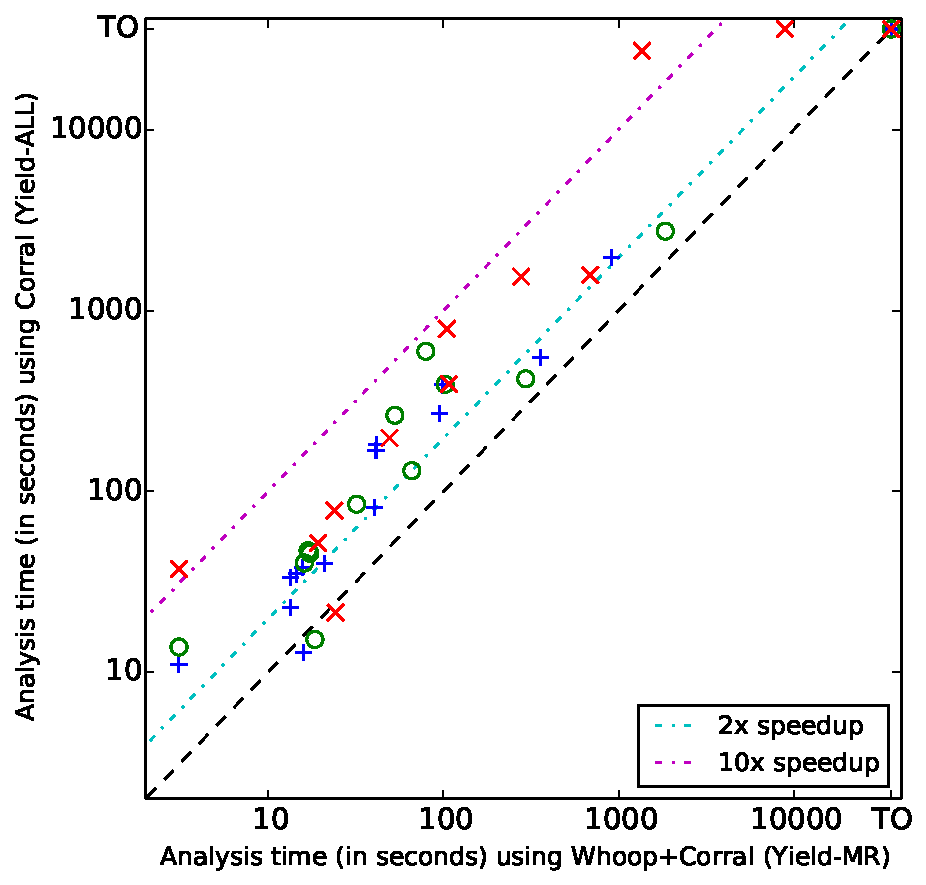
\includegraphics[width=.99\linewidth]{experiments/figures/yieldmr_vs_yieldall.pdf}
\caption{Scatter plot showing the runtime speedups that \corral achieves using \whoop with the \yieldmr instrumentation. The symbols $+$, $\circ$ and $\times$, represent a context-switch bound of 2, 5 and 9, respectively.}
\label{fig:plot}
\end{figure}

We performed experiments to validate the usefulness of the \whoop approach (\S\ref{whoop}) and its combination with \corral (\S\ref{corral}). We first present race-checking results from running \whoop and \corral on \sizeOfBenchmarks drivers taken from the 4.0 Linux kernel distribution.\footnote{\url{https://www.kernel.org}} We then evaluate the runtime performance and scalability of \corral and \whoop + \corral with different yield instrumentation granularities and context-switch bounds.
Our results demonstrate that \whoop can efficiently accelerate race-checking with \corral.

\noindent\textbf{Experimental Setup }
%
We performed all experiments on a 3.40GHz Intel Core i7-2600 CPU with 16GB RAM running Ubuntu Linux 12.04.5 LTS, LLVM 3.5, SMACK 1.5, Z3~4.3.2, Boogie rev. 4192 and \corral rev. 534. We also used Mono~4.1.0 to run Boogie and \corral.

\noindent\textbf{Benchmarks }
%
We evaluate our methodology against \sizeOfBenchmarks drivers taken from the 4.0 Linux kernel. We chose non-trivial drivers from several categories: block; char; ethernet; near field communication (nfc); universal serial bus (usb); and watchdog. We had to manually model the environment for these drivers, a process that required approximately two months of work.

\noindent\textbf{Race-Checking }
%
Table~\ref{tab:stats} presents statistics for all our benchmarks: lines of code (LoC); number of entry point pairs (\#Pairs); number of SMACK memory regions (\#MRs); number of racy pairs reported by \whoop (\#Racy Pairs); number of racy memory regions identified by \whoop (\#Racy MRs); and number of races discovered by \corral using a context-switch bound (csb) of 2 (\#Races Found). Using a higher csb did not uncover any further races; this might mean that races in our benchmarks require only one or two context-switches to manifest, or that \corral hit its bounds before discovering a deeper bug. \corral did not discover any races that \whoop did not already report.  This is expected, as \whoop aims for soundness, and increases our confidence in the implementation of \whoop.

We can see that \whoop reports more races than \corral. This is expected, since \whoop employs an over-approximating shared state abstraction to conservatively model the effects of additional threads when analyzing an entry point pair, and because lockset analysis is inherently imprecise; both factors can lead to false positives.  On the other hand, \corral is precise, but can miss races because only a limited number of context-switches are considered.  Another issue with \corral is loop coverage due to unsound loop unrolling. To tackle this, we enable the built-in loop over-approximation described in~\cite{lal2014powering}. This can potentially lead \corral to report false bugs, but we have not seen this in practice. Finally, when we apply \corral to a pair of entry points, we just check the specific pair and do not account for the effects of other threads (see \S\ref{corral}); this can also cause \corral to miss some races.

Most of the races that \whoop and \corral discovered can be classified in two cases. The first case is accessing a global counter (or flag) from concurrent entry points, without a lock. This might be for performance, and indeed a lot of the races we found might be benign. Even benign races, though, lead to undefined behavior according to the C standard, and it is well known that undefined behaviors can lead to unexpected results when combined with aggressive compiler optimizations. The second case is an entry point accessing a field of an object (either global or passed as a parameter) without a lock. This can lead to a race if another entry point simultaneously accesses the same field of the same object.

As an example of the second case, we found the following race in the generic\_nvram char driver (see Figure~\ref{fig:data_race_example} for the source code): during the \texttt{llseek} entry point, the driver is accessing the file offset \texttt{file->f\_pos} without first acquiring a lock (\texttt{file} is passed as a parameter to \texttt{llseek}). This can lead to a race if the driver invokes \texttt{llseek} from another thread passing the same \texttt{file} object as a parameter. When we investigated another char driver that uses the same APIs, we saw that it was protecting the offset access in its \texttt{llseek} entry point with a mutex. This made us suspicious that the race we found in generic\_nvram could be real. We filed a bug report, but did not manage to get a response yet.

\noindent\textbf{Granularity of Context-Switches }
%
Table~\ref{tab:results} presents runtime results from using \whoop, \corral and \whoop + \corral to analyze our benchmarks, while Figure~\ref{fig:plot} plots the runtime speedups that \corral achieves using \whoop with the \yieldmr instrumentation. All reported times, in seconds, are averages over three runs. \corral was configured with a time budget of 10 hours (T.O. denotes timeout) and a csb of 2, 5 and 9, respectively. For standalone \corral we enable the \yieldall instrumentation, which instruments context-switches (i.e. \texttt{yield} statements) after all visible operations. \whoop + \corral, instead, uses two different context-switch instrumentation granularities, \yieldcoarse and \yieldmr (see \S\ref{corral}). The table also shows the number of context-switches per instrumentation (\#Y).

\whoop uses over-approximation to achieve scalability and, as expected, executes significantly faster than \corral in all our benchmarks. For example, \corral times out in all configurations (without and without \whoop) when trying to analyze the r8169 ethernet driver, while \whoop manages to analyze the driver in 144.5 seconds. We believe that the reason behind this is that r8169 has deeply-nested recursion in some of its entry points, which might get \corral stuck. This is not an issue for \whoop, which uses procedure summarization. This shows that \whoop has value as a stand-alone analyzer.

Using the race-freedom guarantees from \whoop, we managed to significantly accelerate \corral in most of our benchmarks; the best results were achieved using \yieldmr. Figure~\ref{fig:plot} shows that most speedups using \yieldmr are in the range of 1.5--10$\times$; while in ssu100, and pc8736x\_gpio respectively, we achieved a speedup of 12$\times$, and 20$\times$ respectively, using a csb of 9. We notice that a higher csb typically results into greater speedups, when exploiting \whoop. This is expected, as a higher csb directly translates into a larger sequentialized program, and thus \whoop has more opportunities to reduce the sequentialization.

However, if \whoop fails to verify any race-related properties of a driver, it might actually slow down \corral. We noticed this in the sx8 driver, where \whoop does not verify any pairs, causing unnecessary overhead. Although \whoop verified 46 out of 47 memory regions, it still fails to speedup \corral using \yieldmr. This might be because \corral verifies the only 2 pairs of sx8 quite fast (21.4 seconds with csb of 9), and thus the overhead of using \whoop overwhelms any benefits from our fine-grained instrumentation.

\noindent\textbf{Other Tools }
%
We tried to compare \whoop with other similar approaches (see \S\ref{related}). However, we found this hard to achieve, as some tools are not freely available, while others are outdated for several years and are not working on the 4.0 Linux drivers.
